\begin{comment}
\chapter{Complete search}

\key{Complete search}
is a general method that can be used
to solve almost any algorithm problem.
The idea is to generate all possible
solutions to the problem using brute force,
and then select the best solution or count the
number of solutions, depending on the problem.

Complete search is a good technique
if there is enough time to go through all the solutions,
because the search is usually easy to implement
and it always gives the correct answer.
If complete search is too slow,
other techniques, such as greedy algorithms or
dynamic programming, may be needed.
\end{comment}

\chapter{全探索}

全探索(\key{Complete search})はほとんどのアルゴリズムの
問題を解くことができる手段である。
そのアイデアは、あり得る可能性を総当たりですべて列挙し、
その中で問題に応じて最適値を求めたり組み合わせの総数を
求めたりするというものである。

全探索は一般的に実装が容易であり、かつ正しい解にたどり着きやすいため、
十分な時間があるならば良いテクニックである。
全探索では遅すぎる場合は、別のテクニック、例えば
貪欲法なり動的計画法なりが必要となる。


\begin{comment}
\section{Generating subsets}

\index{subset}

We first consider the problem of generating
all subsets of a set of $n$ elements.
For example, the subsets of $\{0,1,2\}$ are
$\emptyset$, $\{0\}$, $\{1\}$, $\{2\}$, $\{0,1\}$,
$\{0,2\}$, $\{1,2\}$ and $\{0,1,2\}$.
There are two common methods to generate subsets:
we can either perform a recursive search
or exploit the bit representation of integers.
\end{comment}

\section{部分集合の生成}

\index{subset}
\index{部分集合}

まず$n$要素の集合から、あり得る全部分集合を列挙する問題を考えよう。
例えば$\{0,1,2\}$の部分集合は
$\emptyset$, $\{0\}$, $\{1\}$, $\{2\}$, $\{0,1\}$,
$\{0,2\}$, $\{1,2\}$, $\{0,1,2\}$である。
部分集合の生成には2つの定番手法として
再帰的な探索と、ビット演算の活用がある。


\begin{comment}
\subsubsection{Method 1}

An elegant way to go through all subsets
of a set is to use recursion.
The following function \texttt{search}
generates the subsets of the set
$\{0,1,\ldots,n-1\}$.
The function maintains a vector \texttt{subset}
that will contain the elements of each subset.
The search begins when the function is called
with parameter 0.

\begin{lstlisting}
void search(int k) {
    if (k == n) {
        // process subset
    } else {
        search(k+1);
        subset.push_back(k);
        search(k+1);
        subset.pop_back();
    }
}
\end{lstlisting}
\end{comment}

\subsubsection{方法 1}

全部分集合を探索するエレガントな方法として
再帰を用いる方法がある。
以下の\texttt{search}関数は集合$\{0,1,\ldots,n-1\}$の
部分集合を生成する。

この.関数は、部分集合の要素を含む配列\texttt{subset}
を管理していく。
探索はこの関数を引数0で呼び出して始める:

\begin{lstlisting}
void search(int k) {
    if (k == n) {
        // 部分集合に関して処理を行う
    } else {
        search(k+1);
        subset.push_back(k);
        search(k+1);
        subset.pop_back();
    }
}
\end{lstlisting}

\begin{comment}
When the function \texttt{search}
is called with parameter $k$,
it decides whether to include the
element $k$ in the subset or not,
and in both cases,
then calls itself with parameter $k+1$
However, if $k=n$, the function notices that
all elements have been processed
and a subset has been generated.

The following tree illustrates the function calls when $n=3$.
We can always choose either the left branch
($k$ is not included in the subset) or the right branch
($k$ is included in the subset).
\end{comment}

関数\texttt{search}が引数$k$で呼び出されると、
その際に部分集合の要素として$k$を含む場合と
含まない場合を考慮し、それぞれに対して
引数を$k+1$として再帰的に処理を行う。
$k=n$となると$n$未満の全要素について
処理が終わったことがわかるので、その時点で
部分集合が生成されたと判断できる。

以下の樹形図は、$n=3$の場合の関数呼び出しを表したものである。
この関数は常に左側の枝($k$が部分集合に含まれない)を探索したのち
右側の枝($k$が部分集合に含まれる)を探索する。

\begin{center}
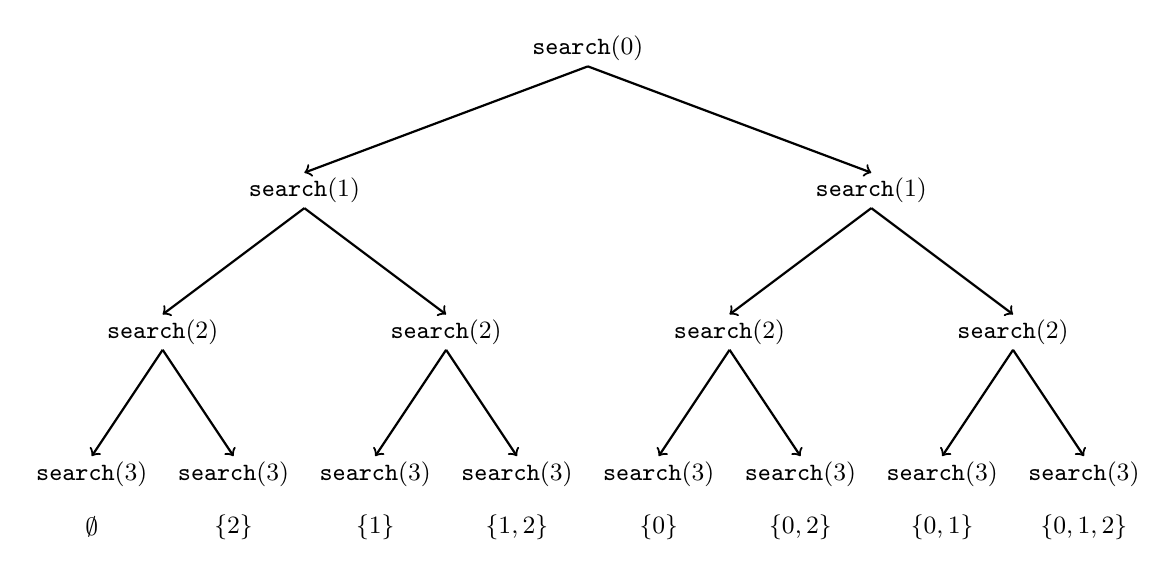
\begin{tikzpicture}[scale=.45]
  \begin{scope}
    \small
    \node at (0,0) {$\texttt{search}(0)$};

    \node at (-8,-4) {$\texttt{search}(1)$};
    \node at (8,-4) {$\texttt{search}(1)$};

    \path[draw,thick,->] (0,0-0.5) -- (-8,-4+0.5);
    \path[draw,thick,->] (0,0-0.5) -- (8,-4+0.5);

    \node at (-12,-8) {$\texttt{search}(2)$};
    \node at (-4,-8) {$\texttt{search}(2)$};
    \node at (4,-8) {$\texttt{search}(2)$};
    \node at (12,-8) {$\texttt{search}(2)$};

    \path[draw,thick,->] (-8,-4-0.5) -- (-12,-8+0.5);
    \path[draw,thick,->] (-8,-4-0.5) -- (-4,-8+0.5);
    \path[draw,thick,->] (8,-4-0.5) -- (4,-8+0.5);
    \path[draw,thick,->] (8,-4-0.5) -- (12,-8+0.5);

    \node at (-14,-12) {$\texttt{search}(3)$};
    \node at (-10,-12) {$\texttt{search}(3)$};
    \node at (-6,-12) {$\texttt{search}(3)$};
    \node at (-2,-12) {$\texttt{search}(3)$};
    \node at (2,-12) {$\texttt{search}(3)$};
    \node at (6,-12) {$\texttt{search}(3)$};
    \node at (10,-12) {$\texttt{search}(3)$};
    \node at (14,-12) {$\texttt{search}(3)$};

    \node at (-14,-13.5) {$\emptyset$};
    \node at (-10,-13.5) {$\{2\}$};
    \node at (-6,-13.5) {$\{1\}$};
    \node at (-2,-13.5) {$\{1,2\}$};
    \node at (2,-13.5) {$\{0\}$};
    \node at (6,-13.5) {$\{0,2\}$};
    \node at (10,-13.5) {$\{0,1\}$};
    \node at (14,-13.5) {$\{0,1,2\}$};


    \path[draw,thick,->] (-12,-8-0.5) -- (-14,-12+0.5);
    \path[draw,thick,->] (-12,-8-0.5) -- (-10,-12+0.5);
    \path[draw,thick,->] (-4,-8-0.5) -- (-6,-12+0.5);
    \path[draw,thick,->] (-4,-8-0.5) -- (-2,-12+0.5);
    \path[draw,thick,->] (4,-8-0.5) -- (2,-12+0.5);
    \path[draw,thick,->] (4,-8-0.5) -- (6,-12+0.5);
    \path[draw,thick,->] (12,-8-0.5) -- (10,-12+0.5);
    \path[draw,thick,->] (12,-8-0.5) -- (14,-12+0.5);
\end{scope}
\end{tikzpicture}
\end{center}

\begin{comment}
\subsubsection{Method 2}

Another way to generate subsets is based on
the bit representation of integers.
Each subset of a set of $n$ elements
can be represented as a sequence of $n$ bits,
which corresponds to an integer between $0 \ldots 2^n-1$.
The ones in the bit sequence indicate
which elements are included in the subset.

The usual convention is that
the last bit corresponds to element 0,
the second last bit corresponds to element 1,
and so on.
For example, the bit representation of 25
is 11001, which corresponds to the subset $\{0,3,4\}$.
\end{comment}

\subsubsection{方法 2}

部分集合群を生成する別の方法は、整数におけるビット表現を
活用することである。
$n$要素の集合の部分集合を$n$ビットの並びとして表現する。
すなわち$0 \ldots 2^n-1$の範囲の整数に対応付ける。
ビット列中1がセットされた箇所は、対応する要素が部分集合中に
含まれていることを意味する。

良くある対応付けは、末尾のビットを要素0、末尾から2番目のビットを
要素1、というように対応付けるものである。
例えば整数値25のビット表現は11001となるが、
これは部分集合$\{0,3,4\}$と対応付けられる。

\begin{comment}
The following code goes through the subsets
of a set of $n$ elements

\begin{lstlisting}
for (int b = 0; b < (1<<n); b++) {
    // process subset
}
\end{lstlisting}

The following code shows how we can find
the elements of a subset that corresponds to a bit sequence.
When processing each subset,
the code builds a vector that contains the
elements in the subset.
\end{comment}

$n$要素の部分集合群は、以下のコードで探索できる:

\begin{lstlisting}
for (int b = 0; b < (1<<n); b++) {
    // 部分集合を処理する
}
\end{lstlisting}

以下のコードは、ビット列に対応する部分集合の生成法を示している。
各部分集合を示すビット列に対応して、実際の要素を
含む配列を生成している。

\begin{lstlisting}
for (int b = 0; b < (1<<n); b++) {
    vector<int> subset;
    for (int i = 0; i < n; i++) {
        if (b&(1<<i)) subset.push_back(i);
    }
}
\end{lstlisting}

\begin{comment}
\section{Generating permutations}

\index{permutation}

Next we consider the problem of generating
all permutations of a set of $n$ elements.
For example, the permutations of $\{0,1,2\}$ are
$(0,1,2)$, $(0,2,1)$, $(1,0,2)$, $(1,2,0)$,
$(2,0,1)$ and $(2,1,0)$.
Again, there are two approaches:
we can either use recursion or go through the
permutations iteratively.

\end{comment}

\section{順列の生成}

\index{permutation}
\index{順列}

続けて、$n$要素のすべての順列を生成する問題を考える。
例えば、$\{0,1,2\}$の順列は$(0,1,2)$, $(0,2,1)$, $(1,0,2)$, $(1,2,0)$,
$(2,0,1)$,$(2,1,0)$である。
こちらも2つの定番アプローチとして、再帰を用いる方法と
順次順列を生成していく方法がある。

\begin{comment}
\subsubsection{Method 1}

Like subsets, permutations can be generated
using recursion.
The following function \texttt{search} goes
through the permutations of the set $\{0,1,\ldots,n-1\}$.
The function builds a vector \texttt{permutation}
that contains the permutation,
and the search begins when the function is
called without parameters.

\begin{lstlisting}
void search() {
    if (permutation.size() == n) {
        // process permutation
    } else {
        for (int i = 0; i < n; i++) {
            if (chosen[i]) continue;
            chosen[i] = true;
            permutation.push_back(i);
            search();
            chosen[i] = false;
            permutation.pop_back();
        }
    }
}
\end{lstlisting}
\end{comment}

\subsubsection{方法 1}

部分集合同様、順列も再帰を使って生成できる。
以下の関数\texttt{search}は集合$\{0,1,\ldots,n-1\}$の順列を生成し、
配列\texttt{permutation}に格納していく。
この再帰関数は、配列が空の状態で始まる:

\begin{lstlisting}
void search() {
    if (permutation.size() == n) {
        // 順列に関し処理を行う
    } else {
        for (int i = 0; i < n; i++) {
            if (chosen[i]) continue;
            chosen[i] = true;
            permutation.push_back(i);
            search();
            chosen[i] = false;
            permutation.pop_back();
        }
    }
}
\end{lstlisting}

\begin{comment}
Each function call adds a new element to
\texttt{permutation}.
The array \texttt{chosen} indicates which
elements are already included in the permutation.
If the size of \texttt{permutation} equals the size of the set,
a permutation has been generated.
\end{comment}

関数が呼び出されるたびに\texttt{permutation}に
要素が追加されていく。
配列\texttt{chosen}は、どの要素がすでに順列に
含まれているかを示す。
\texttt{permutation}の大きさが元の集合と一致すると
処理は完了し、順列が生成された状態となる。

\begin{comment}
\subsubsection{Method 2}

\index{next\_permutation@\texttt{next\_permutation}}

Another method for generating permutations
is to begin with the permutation
$\{0,1,\ldots,n-1\}$ and repeatedly
use a function that constructs the next permutation
in increasing order.
The C++ standard library contains the function
\texttt{next\_permutation} that can be used for this:

\begin{lstlisting}
vector<int> permutation;
for (int i = 0; i < n; i++) {
    permutation.push_back(i);
}
do {
    // process permutation
} while (next_permutation(permutation.begin(),permutation.end()));
\end{lstlisting}
\end{comment}

\subsubsection{方法 2}

\index{next\_permutation@\texttt{next\_permutation}}

順列を生成する別の方法は、まず$\{0,1,\ldots,n-1\}$から初めて、
辞書順で次の順列を順次生成していく方法である。
C++標準ライブラリにある\texttt{next\_permutation}関数が
この手続きを提供している:

\begin{lstlisting}
vector<int> permutation;
for (int i = 0; i < n; i++) {
    permutation.push_back(i);
}
do {
    // 処理を行う
} while (next_permutation(permutation.begin(),permutation.end()));
\end{lstlisting}

\begin{comment}
\section{Backtracking}

\index{backtracking}

A \key{backtracking} algorithm
begins with an empty solution
and extends the solution step by step.
The search recursively
goes through all different ways how
a solution can be constructed.
\end{comment}

\section{バックトラック法}

\index{backtracking}
\index{バックトラック法}

バックトラック法(\key{backtracking})とは、
初期状態から1手ずつ再帰的に先に進めていき、
最終的に異なる状態をすべてたどる方法である。

\begin{comment}
\index{queen problem}

As an example, consider the problem of
calculating the number
of ways $n$ queens can be placed on
an $n \times n$ chessboard so that
no two queens attack each other.
For example, when $n=4$,
there are two possible solutions:
\end{comment}

\index{queen problem}
\index{Nクイーン問題}

例として、$n \times n$の大きさのチェス盤に
$n$個のクイーンの駒を互いに攻撃できない位置に
置く置き方を数え上げる問題を考える。
例えば$n=4$の場合次の2つの解がある:

\begin{center}
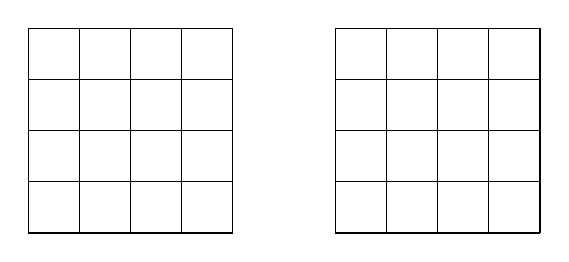
\begin{tikzpicture}[scale=.65]
  \begin{scope}
    \draw (0, 0) grid (4, 4);
    \node at (1.5,3.5) {\symqueen};
    \node at (3.5,2.5) {\symqueen};
    \node at (0.5,1.5) {\symqueen};
    \node at (2.5,0.5) {\symqueen};

    \draw (6, 0) grid (10, 4);
    \node at (6+2.5,3.5) {\symqueen};
    \node at (6+0.5,2.5) {\symqueen};
    \node at (6+3.5,1.5) {\symqueen};
    \node at (6+1.5,0.5) {\symqueen};

  \end{scope}
\end{tikzpicture}
\end{center}

\begin{comment}
The problem can be solved using backtracking
by placing queens to the board row by row.
More precisely, exactly one queen will
be placed on each row so that no queen attacks
any of the queens placed before.
A solution has been found when all
$n$ queens have been placed on the board.

For example, when $n=4$,
some partial solutions generated by
the backtracking algorithm are as follows:
\end{comment}

この問題は行ごとに駒を配置していくバックトラック法で
解くことができる。
より正確に書くと、各列にすでに置いた駒と互いに攻撃
しあわないような位置に新たに1箇所駒を追加していく。
$n$個の駒をすべて配置したらそれが解となる。

例えば$n=4$の場合、バックトラック法で生成される
解の一部は下記の通りとなる:

\begin{comment}
\begin{center}
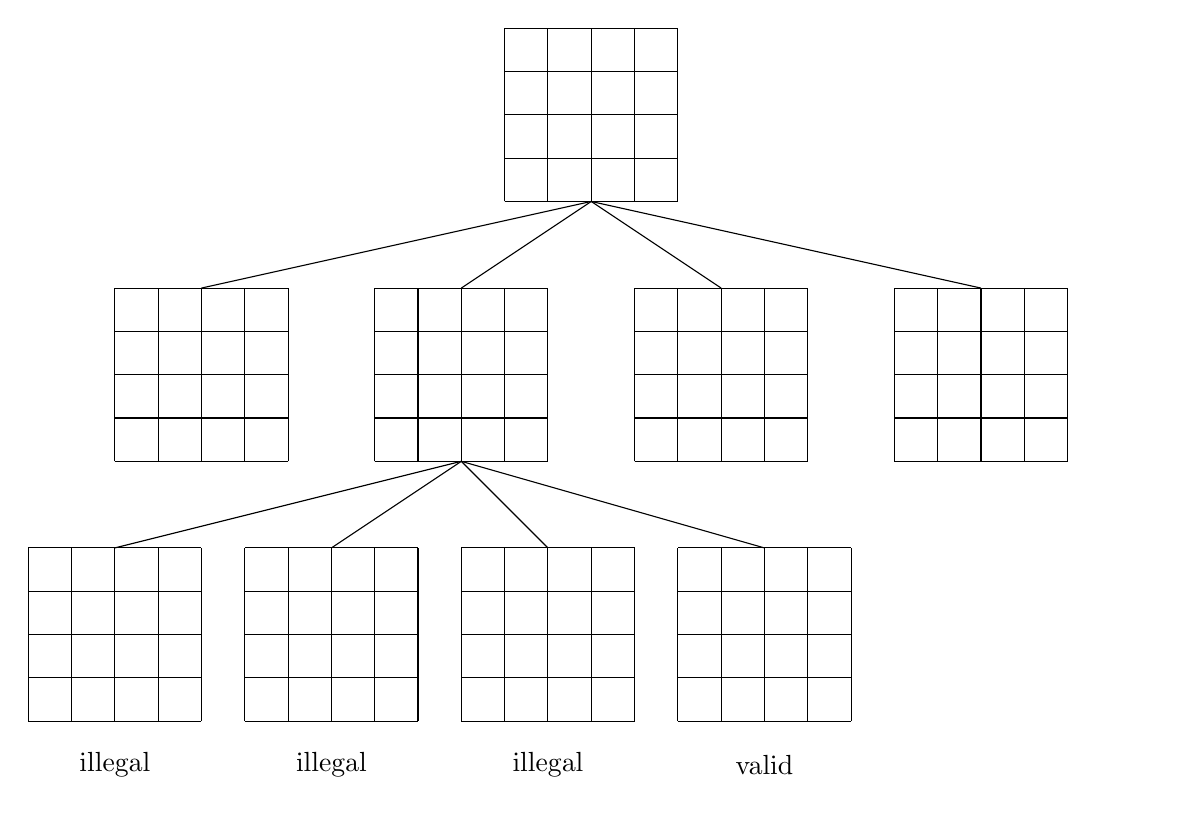
\begin{tikzpicture}[scale=.55]
  \begin{scope}
    \draw (0, 0) grid (4, 4);

    \draw (-9, -6) grid (-5, -2);
    \draw (-3, -6) grid (1, -2);
    \draw (3, -6) grid (7, -2);
    \draw (9, -6) grid (13, -2);

    \node at (-9+0.5,-3+0.5) {\symqueen};
    \node at (-3+1+0.5,-3+0.5) {\symqueen};
    \node at (3+2+0.5,-3+0.5) {\symqueen};
    \node at (9+3+0.5,-3+0.5) {\symqueen};

    \draw (2,0) -- (-7,-2);
    \draw (2,0) -- (-1,-2);
    \draw (2,0) -- (5,-2);
    \draw (2,0) -- (11,-2);

    \draw (-11, -12) grid (-7, -8);
    \draw (-6, -12) grid (-2, -8);
    \draw (-1, -12) grid (3, -8);
    \draw (4, -12) grid (8, -8);
    \draw[white] (11, -12) grid (15, -8);
    \node at (-11+1+0.5,-9+0.5) {\symqueen};
    \node at (-6+1+0.5,-9+0.5) {\symqueen};
    \node at (-1+1+0.5,-9+0.5) {\symqueen};
    \node at (4+1+0.5,-9+0.5) {\symqueen};
    \node at (-11+0+0.5,-10+0.5) {\symqueen};
    \node at (-6+1+0.5,-10+0.5) {\symqueen};
    \node at (-1+2+0.5,-10+0.5) {\symqueen};
    \node at (4+3+0.5,-10+0.5) {\symqueen};

    \draw (-1,-6) -- (-9,-8);
    \draw (-1,-6) -- (-4,-8);
    \draw (-1,-6) -- (1,-8);
    \draw (-1,-6) -- (6,-8);

    \node at (-9,-13) {illegal};
    \node at (-4,-13) {illegal};
    \node at (1,-13) {illegal};
    \node at (6,-13) {valid};

  \end{scope}
\end{tikzpicture}
\end{center}
\end{comment}

\begin{center}
\begin{tikzpicture}[scale=.55]
  \begin{scope}
    \draw (0, 0) grid (4, 4);

    \draw (-9, -6) grid (-5, -2);
    \draw (-3, -6) grid (1, -2);
    \draw (3, -6) grid (7, -2);
    \draw (9, -6) grid (13, -2);

    \node at (-9+0.5,-3+0.5) {\symqueen};
    \node at (-3+1+0.5,-3+0.5) {\symqueen};
    \node at (3+2+0.5,-3+0.5) {\symqueen};
    \node at (9+3+0.5,-3+0.5) {\symqueen};

    \draw (2,0) -- (-7,-2);
    \draw (2,0) -- (-1,-2);
    \draw (2,0) -- (5,-2);
    \draw (2,0) -- (11,-2);

    \draw (-11, -12) grid (-7, -8);
    \draw (-6, -12) grid (-2, -8);
    \draw (-1, -12) grid (3, -8);
    \draw (4, -12) grid (8, -8);
    \draw[white] (11, -12) grid (15, -8);
    \node at (-11+1+0.5,-9+0.5) {\symqueen};
    \node at (-6+1+0.5,-9+0.5) {\symqueen};
    \node at (-1+1+0.5,-9+0.5) {\symqueen};
    \node at (4+1+0.5,-9+0.5) {\symqueen};
    \node at (-11+0+0.5,-10+0.5) {\symqueen};
    \node at (-6+1+0.5,-10+0.5) {\symqueen};
    \node at (-1+2+0.5,-10+0.5) {\symqueen};
    \node at (4+3+0.5,-10+0.5) {\symqueen};

    \draw (-1,-6) -- (-9,-8);
    \draw (-1,-6) -- (-4,-8);
    \draw (-1,-6) -- (1,-8);
    \draw (-1,-6) -- (6,-8);

    \node at (-9,-13) {無効};
    \node at (-4,-13) {無効};
    \node at (1,-13) {無効};
    \node at (6,-13) {有効};

  \end{scope}
\end{tikzpicture}
\end{center}

\begin{comment}
At the bottom level, the three first configurations
are illegal, because the queens attack each other.
However, the fourth configuration is valid
and it can be extended to a complete solution by
placing two more queens to the board.
There is only one way to place the two remaining queens.
\end{comment}


図における最下段の4通りの例において、先頭の3つの構成はクイーンが互いに互いを攻撃できるため無効である。
しかし4つ目の構成は有効であり、残り2つのクイーンを置いていくと完全な解まで探索を
拡張できる。
残り2つのクイーンの置き方は一通りしかない。


\begin{samepage}

\begin{comment}
The algorithm can be implemented as follows:
\end{comment}

このアルゴリズムはこのように実装できる:
\begin{lstlisting}
void search(int y) {
    if (y == n) {
        count++;
        return;
    }
    for (int x = 0; x < n; x++) {
        if (column[x] || diag1[x+y] || diag2[x-y+n-1]) continue;
        column[x] = diag1[x+y] = diag2[x-y+n-1] = 1;
        search(y+1);
        column[x] = diag1[x+y] = diag2[x-y+n-1] = 0;
    }
}
\end{lstlisting}
\end{samepage}

\begin{comment}
The search begins by calling \texttt{search(0)}.
The size of the board is $n \times n$,
and the code calculates the number of solutions
to \texttt{count}.

The code assumes that the rows and columns
of the board are numbered from 0 to $n-1$.
When the function \texttt{search} is
called with parameter $y$,
it places a queen on row $y$
and then calls itself with parameter $y+1$.
Then, if $y=n$, a solution has been found
and the variable \texttt{count} is increased by one.

The array \texttt{column} keeps track of columns
that contain a queen,
and the arrays \texttt{diag1} and \texttt{diag2}
keep track of diagonals.
It is not allowed to add another queen to a
column or diagonal that already contains a queen. 
For example, the columns and diagonals of
the $4 \times 4$ board are numbered as follows:

\end{comment}

この探索は\texttt{search(0)}を呼ぶことで開始する。
盤面の大きさを$n$とすると、このコードは求める解を計算し
\texttt{count}に格納する。

このコードでは、列および行が0から$n-1$まで番号が振られているものとして
計算を行う。

関数\texttt{search}が引数$y$を伴って呼び出されると、
この関数は$y$行目にクイーンを1つ置き、
自身の関数を引数$y+1$として再帰的に呼び出す。
そのため、$y=n$に到達すると、解が1つ見つかったとみなすことができ、
変数\texttt{count}がインクリメントされる。

配列\texttt{column}はクイーンが配置された列の情報を
保存するものであり、配列\texttt{diag1}と\texttt{diag2}は
クイーンが配置された斜め方向の列の情報を保存するものである。
すでにクイーンの配置された列や対角上にクイーンを追加することはできない。
例えば、$4 \times 4$の盤面上を以下のように番号を割り当てる:

\begin{comment}
\begin{center}
\begin{tikzpicture}[scale=.65]
  \begin{scope}
    \draw (0-6, 0) grid (4-6, 4);
    \node at (-6+0.5,3.5) {$0$};
    \node at (-6+1.5,3.5) {$1$};
    \node at (-6+2.5,3.5) {$2$};
    \node at (-6+3.5,3.5) {$3$};
    \node at (-6+0.5,2.5) {$0$};
    \node at (-6+1.5,2.5) {$1$};
    \node at (-6+2.5,2.5) {$2$};
    \node at (-6+3.5,2.5) {$3$};
    \node at (-6+0.5,1.5) {$0$};
    \node at (-6+1.5,1.5) {$1$};
    \node at (-6+2.5,1.5) {$2$};
    \node at (-6+3.5,1.5) {$3$};
    \node at (-6+0.5,0.5) {$0$};
    \node at (-6+1.5,0.5) {$1$};
    \node at (-6+2.5,0.5) {$2$};
    \node at (-6+3.5,0.5) {$3$};

    \draw (0, 0) grid (4, 4);
    \node at (0.5,3.5) {$0$};
    \node at (1.5,3.5) {$1$};
    \node at (2.5,3.5) {$2$};
    \node at (3.5,3.5) {$3$};
    \node at (0.5,2.5) {$1$};
    \node at (1.5,2.5) {$2$};
    \node at (2.5,2.5) {$3$};
    \node at (3.5,2.5) {$4$};
    \node at (0.5,1.5) {$2$};
    \node at (1.5,1.5) {$3$};
    \node at (2.5,1.5) {$4$};
    \node at (3.5,1.5) {$5$};
    \node at (0.5,0.5) {$3$};
    \node at (1.5,0.5) {$4$};
    \node at (2.5,0.5) {$5$};
    \node at (3.5,0.5) {$6$};

    \draw (6, 0) grid (10, 4);
    \node at (6.5,3.5) {$3$};
    \node at (7.5,3.5) {$4$};
    \node at (8.5,3.5) {$5$};
    \node at (9.5,3.5) {$6$};
    \node at (6.5,2.5) {$2$};
    \node at (7.5,2.5) {$3$};
    \node at (8.5,2.5) {$4$};
    \node at (9.5,2.5) {$5$};
    \node at (6.5,1.5) {$1$};
    \node at (7.5,1.5) {$2$};
    \node at (8.5,1.5) {$3$};
    \node at (9.5,1.5) {$4$};
    \node at (6.5,0.5) {$0$};
    \node at (7.5,0.5) {$1$};
    \node at (8.5,0.5) {$2$};
    \node at (9.5,0.5) {$3$};

    \node at (-4,-1) {\texttt{column}};
    \node at (2,-1) {\texttt{diag1}};
    \node at (8,-1) {\texttt{diag2}};
\end{comment}

\begin{center}
\begin{tikzpicture}[scale=.65]
  \begin{scope}
    \draw (0-6, 0) grid (4-6, 4);
    \node at (-6+0.5,3.5) {$0$};
    \node at (-6+1.5,3.5) {$1$};
    \node at (-6+2.5,3.5) {$2$};
    \node at (-6+3.5,3.5) {$3$};
    \node at (-6+0.5,2.5) {$0$};
    \node at (-6+1.5,2.5) {$1$};
    \node at (-6+2.5,2.5) {$2$};
    \node at (-6+3.5,2.5) {$3$};
    \node at (-6+0.5,1.5) {$0$};
    \node at (-6+1.5,1.5) {$1$};
    \node at (-6+2.5,1.5) {$2$};
    \node at (-6+3.5,1.5) {$3$};
    \node at (-6+0.5,0.5) {$0$};
    \node at (-6+1.5,0.5) {$1$};
    \node at (-6+2.5,0.5) {$2$};
    \node at (-6+3.5,0.5) {$3$};

    \draw (0, 0) grid (4, 4);
    \node at (0.5,3.5) {$0$};
    \node at (1.5,3.5) {$1$};
    \node at (2.5,3.5) {$2$};
    \node at (3.5,3.5) {$3$};
    \node at (0.5,2.5) {$1$};
    \node at (1.5,2.5) {$2$};
    \node at (2.5,2.5) {$3$};
    \node at (3.5,2.5) {$4$};
    \node at (0.5,1.5) {$2$};
    \node at (1.5,1.5) {$3$};
    \node at (2.5,1.5) {$4$};
    \node at (3.5,1.5) {$5$};
    \node at (0.5,0.5) {$3$};
    \node at (1.5,0.5) {$4$};
    \node at (2.5,0.5) {$5$};
    \node at (3.5,0.5) {$6$};

    \draw (6, 0) grid (10, 4);
    \node at (6.5,3.5) {$3$};
    \node at (7.5,3.5) {$4$};
    \node at (8.5,3.5) {$5$};
    \node at (9.5,3.5) {$6$};
    \node at (6.5,2.5) {$2$};
    \node at (7.5,2.5) {$3$};
    \node at (8.5,2.5) {$4$};
    \node at (9.5,2.5) {$5$};
    \node at (6.5,1.5) {$1$};
    \node at (7.5,1.5) {$2$};
    \node at (8.5,1.5) {$3$};
    \node at (9.5,1.5) {$4$};
    \node at (6.5,0.5) {$0$};
    \node at (7.5,0.5) {$1$};
    \node at (8.5,0.5) {$2$};
    \node at (9.5,0.5) {$3$};

    \node at (-4,-1) {\texttt{列}};
    \node at (2,-1) {\texttt{対角1}};
    \node at (8,-1) {\texttt{対角2}};

  \end{scope}
\end{tikzpicture}
\end{center}

\begin{comment}
Let $q(n)$ denote the number of ways
to place $n$ queens on an $n \times n$ chessboard.
The above backtracking
algorithm tells us that, for example, $q(8)=92$.
When $n$ increases, the search quickly becomes slow,
because the number of solutions increases
exponentially.
For example, calculating $q(16)=14772512$
using the above algorithm already takes about a minute
on a modern computer\footnote{There is no known way to efficiently
calculate larger values of $q(n)$. The current record is
$q(27)=234907967154122528$, calculated in 2016 \cite{q27}.}.
\end{comment}

$q(n)$ を $n \times n$ の盤面に $n$ 個のクイーンを置く置き方の総数とする。
先ほどのバックトラッキングにより、例えば $q(8)=92$ であることがわかる。
$n$が増えると、探索は非常に遅くなる。
というのも、総数が指数関数的に大きくなるためである。
例えば、 $q(16)=14772512$ をこの方法で計算すると最近の計算機でも
1分程度かかる。 \footnote{大きな$q(n)$を効率的に計算する手法は知られていない。
現在の記録は、2016年に計算された $q(27)=234907967154122528$ である \cite{q27}。}

\begin{comment}
\section{Pruning the search}

We can often optimize backtracking
by pruning the search tree.
The idea is to add ''intelligence'' to the algorithm
so that it will notice as soon as possible
if a partial solution cannot be extended
to a complete solution.
Such optimizations can have a tremendous
effect on the efficiency of the search.

Let us consider the problem
of calculating the number of paths
in an $n \times n$ grid from the upper-left corner
to the lower-right corner such that the
path visits each square exactly once.
For example, in a $7 \times 7$ grid,
there are 111712 such paths.
One of the paths is as follows:
\end{comment}

\section{探索の枝刈り}

しばしば探索木を枝刈りすることで、バックトラッキングの最適化が可能である。
そのアイデアは、アルゴリズムに判断を加え、今の探索を継続しても求める解に
たどり着きそうにない場合、できるだけ早く気づき探索を打ち切ることである。
このような最適化は探索の効率に著しく影響する場合がある。

ここで、$n \times n$のグリッドにおいて、
左上角のセルから右下角のセルに全セルを1回ずつ通って
到達するパスの組み合わせを求める問題を考えてみよう。

例えば、$7 \times 7$のグリッドにおいてそのようなパスは
111712通りある。下記はその一例である:

\begin{center}
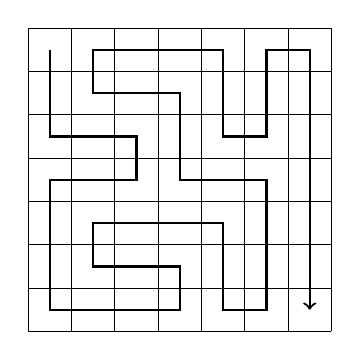
\begin{tikzpicture}[scale=.55]
  \begin{scope}
    \draw (0, 0) grid (7, 7);
    \draw[thick,->] (0.5,6.5) -- (0.5,4.5) -- (2.5,4.5) --
          (2.5,3.5) -- (0.5,3.5) -- (0.5,0.5) --
          (3.5,0.5) -- (3.5,1.5) -- (1.5,1.5) --
          (1.5,2.5) -- (4.5,2.5) -- (4.5,0.5) --
          (5.5,0.5) -- (5.5,3.5) -- (3.5,3.5) --
          (3.5,5.5) -- (1.5,5.5) -- (1.5,6.5) --
          (4.5,6.5) -- (4.5,4.5) -- (5.5,4.5) --
          (5.5,6.5) -- (6.5,6.5) -- (6.5,0.5);
  \end{scope}
\end{tikzpicture}
\end{center}

\begin{comment}
We focus on the $7 \times 7$ case,
because its level of difficulty is appropriate to our needs.
We begin with a straightforward backtracking algorithm,
and then optimize it step by step using observations
of how the search can be pruned.
After each optimization, we measure the running time
of the algorithm and the number of recursive calls,
so that we clearly see the effect of each
optimization on the efficiency of the search.
\end{comment}

以下アルゴリズムを考える上で適度な難易度なので、
$7 \times 7$のケースに着目していく。
まず単純なバックトラッキングアルゴリズムから始め、
そこから探索を枝刈りできるか考察することで
徐々に最適化していこう。


\begin{comment}
\subsubsection{Basic algorithm}

The first version of the algorithm does not contain
any optimizations. We simply use backtracking to generate
all possible paths from the upper-left corner to
the lower-right corner and count the number of such paths.

\begin{itemize}
\item
running time: 483 seconds
\item
number of recursive calls: 76 billion
\end{itemize}
\end{comment}

\subsubsection{基本的なアルゴリズム}

最初のバージョンは、何も最適化せず、単純に可能なパスを全列挙して
その数を数えるものとした。

\begin{itemize}
\item
実行時間: 483秒
\item
再帰呼び出しの回数: 760億回
\end{itemize}

\begin{comment}
\subsubsection{Optimization 1}

In any solution, we first move one step
down or right.
There are always two paths that 
are symmetric
about the diagonal of the grid
after the first step.
For example, the following paths are symmetric:
\end{comment}

\subsubsection{最適化1}

どんな解も、最初のステップは下か右である。
ある解に対して、対角に対して線対称な2つのパスが存在する。
例えば、以下の2つのパスは対称である。

\begin{center}
\begin{tabular}{ccc}
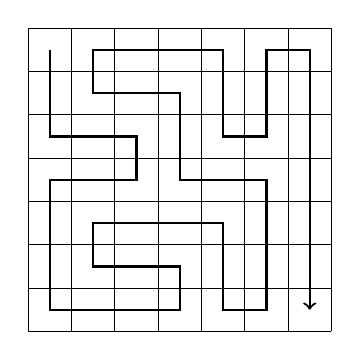
\begin{tikzpicture}[scale=.55]
  \begin{scope}
    \draw (0, 0) grid (7, 7);
    \draw[thick,->] (0.5,6.5) -- (0.5,4.5) -- (2.5,4.5) --
          (2.5,3.5) -- (0.5,3.5) -- (0.5,0.5) --
          (3.5,0.5) -- (3.5,1.5) -- (1.5,1.5) --
          (1.5,2.5) -- (4.5,2.5) -- (4.5,0.5) --
          (5.5,0.5) -- (5.5,3.5) -- (3.5,3.5) --
          (3.5,5.5) -- (1.5,5.5) -- (1.5,6.5) --
          (4.5,6.5) -- (4.5,4.5) -- (5.5,4.5) --
          (5.5,6.5) -- (6.5,6.5) -- (6.5,0.5);
  \end{scope}
\end{tikzpicture}
& \hspace{20pt}
& 
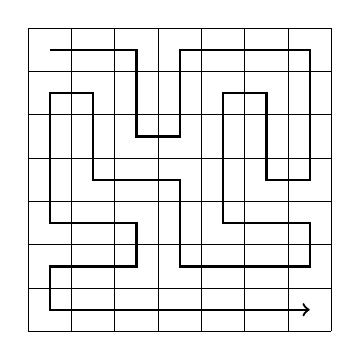
\begin{tikzpicture}[scale=.55]
  \begin{scope}[yscale=1,xscale=-1,rotate=-90]
    \draw (0, 0) grid (7, 7);
    \draw[thick,->] (0.5,6.5) -- (0.5,4.5) -- (2.5,4.5) --
          (2.5,3.5) -- (0.5,3.5) -- (0.5,0.5) --
          (3.5,0.5) -- (3.5,1.5) -- (1.5,1.5) --
          (1.5,2.5) -- (4.5,2.5) -- (4.5,0.5) --
          (5.5,0.5) -- (5.5,3.5) -- (3.5,3.5) --
          (3.5,5.5) -- (1.5,5.5) -- (1.5,6.5) --
          (4.5,6.5) -- (4.5,4.5) -- (5.5,4.5) --
          (5.5,6.5) -- (6.5,6.5) -- (6.5,0.5);
  \end{scope}
\end{tikzpicture}
\end{tabular}
\end{center}

\begin{comment}
Hence, we can decide that we always first
move one step down (or right),
and finally multiply the number of solutions by two.

\begin{itemize}
\item
running time: 244 seconds
\item
number of recursive calls: 38 billion
\end{itemize}
\end{comment}

そのため、最初の移動は下(または右)と決め打ちし、
最後に得られた値を倍にしよう

\begin{itemize}
\item
実行時間: 244 秒
\item
再帰呼び出しの回数: 380億回
\end{itemize}

\begin{comment}
\subsubsection{Optimization 2}

If the path reaches the lower-right square
before it has visited all other squares of the grid,
it is clear that
it will not be possible to complete the solution.
An example of this is the following path:
\end{comment}

\subsubsection{最適化2}

もしパスが全セルを辿る前に右下角に到達してしまった場合、
以後の処理を続けても求めるパスにならないことは明らかである。
以下のパスはその例である:

\begin{center}
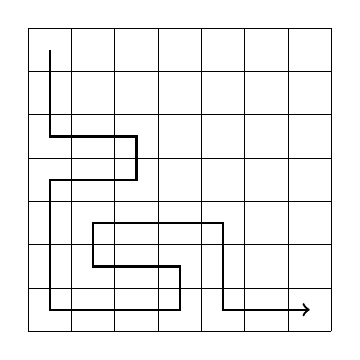
\begin{tikzpicture}[scale=.55]
  \begin{scope}
    \draw (0, 0) grid (7, 7);
    \draw[thick,->] (0.5,6.5) -- (0.5,4.5) -- (2.5,4.5) --
          (2.5,3.5) -- (0.5,3.5) -- (0.5,0.5) --
          (3.5,0.5) -- (3.5,1.5) -- (1.5,1.5) --
          (1.5,2.5) -- (4.5,2.5) -- (4.5,0.5) --
          (6.5,0.5);
  \end{scope}
\end{tikzpicture}
\end{center}

\begin{comment}
Using this observation, we can terminate the search
immediately if we reach the lower-right square too early.
\begin{itemize}
\item
running time: 119 seconds
\item
number of recursive calls: 20 billion
\end{itemize}
\end{comment}

この考察より、右下角に早く到達した場合、
探索を打ち切ることができる。
\begin{itemize}
\item
実行時間: 119 秒
\item
再帰呼び出しの回数: 200億回
\end{itemize}

\begin{comment}
\subsubsection{Optimization 3}

If the path touches a wall
and can turn either left or right,
the grid splits into two parts
that contain unvisited squares.
For example, in the following situation,
the path can turn either left or right:
\end{comment}

\subsubsection{最適化3}

パスが途中で周辺部に到達して、次に左か右に曲がるとき、
グリッドは未到達セルを含む2つのパートに分割される。
例えば、以下の状況では、パスは左か右に曲がることができる。

\begin{center}
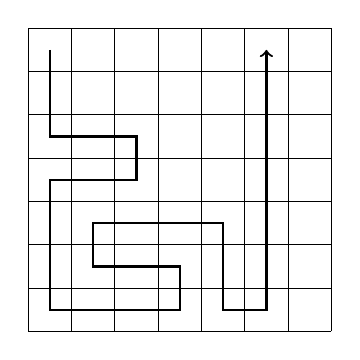
\begin{tikzpicture}[scale=.55]
  \begin{scope}
    \draw (0, 0) grid (7, 7);
    \draw[thick,->] (0.5,6.5) -- (0.5,4.5) -- (2.5,4.5) --
          (2.5,3.5) -- (0.5,3.5) -- (0.5,0.5) --
          (3.5,0.5) -- (3.5,1.5) -- (1.5,1.5) --
          (1.5,2.5) -- (4.5,2.5) -- (4.5,0.5) --
          (5.5,0.5) -- (5.5,6.5);
  \end{scope}
\end{tikzpicture}
\end{center}

\begin{comment}
In this case, we cannot visit all squares anymore,
so we can terminate the search.
This optimization is very useful:

\begin{itemize}
\item
running time: 1.8 seconds
\item
number of recursive calls: 221 million
\end{itemize}
\end{comment}

この例では、もはや全セルを辿ることはできないため、
探索を打ち切ることができる。
この最適化は非常に効果的である:

\begin{itemize}
\item
実行時間: 1.8 秒
\item
再帰呼び出しの回数: 2.21億回
\end{itemize}

\begin{comment}
\subsubsection{Optimization 4}

The idea of Optimization 3
can be generalized:
if the path cannot continue forward
but can turn either left or right,
the grid splits into two parts
that both contain unvisited squares.
For example, consider the following path:
\end{comment}

\subsubsection{最適化4}

最適化3のアイデアをさらに一般化する。
パスが前に伸ばすことができず、左右どちらかに曲げることが可能な場合、
グリッドは2つの未到達パートに分割される。
例えば以下のようなパスを考える:

\begin{center}
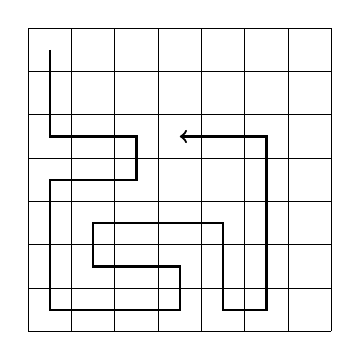
\begin{tikzpicture}[scale=.55]
  \begin{scope}
    \draw (0, 0) grid (7, 7);
    \draw[thick,->] (0.5,6.5) -- (0.5,4.5) -- (2.5,4.5) --
          (2.5,3.5) -- (0.5,3.5) -- (0.5,0.5) --
          (3.5,0.5) -- (3.5,1.5) -- (1.5,1.5) --
          (1.5,2.5) -- (4.5,2.5) -- (4.5,0.5) --
          (5.5,0.5) -- (5.5,4.5) -- (3.5,4.5);
  \end{scope}
\end{tikzpicture}
\end{center}

\begin{comment}
It is clear that we cannot visit all squares anymore,
so we can terminate the search.
After this optimization, the search is
very efficient:

\begin{itemize}
\item
running time: 0.6 seconds
\item
number of recursive calls: 69 million
\end{itemize}
\end{comment}

この例でも、全セルを辿ることができないことは明らかなので、
探索を打ち切ることができる。
この最適化により、探索は非常に効率的になった:

\begin{itemize}
\item
実行時間: 0.6 秒
\item
再帰呼び出しの回数: 6900万回
\end{itemize}


\begin{comment}
~\\
Now is a good moment to stop optimizing
the algorithm and see what we have achieved.
The running time of the original algorithm
was 483 seconds,
and now after the optimizations,
the running time is only 0.6 seconds.
Thus, the algorithm became nearly 1000 times
faster after the optimizations.

This is a usual phenomenon in backtracking,
because the search tree is usually large
and even simple observations can effectively
prune the search.
Especially useful are optimizations that
occur during the first steps of the algorithm,
i.e., at the top of the search tree.
\end{comment}

~\\
この辺で最適化を止め、効果を振り返ってみよう。
元のアルゴリズムの実行時間は483秒だが、
度重なる最適化により、たった0.6秒まで短縮した。
すなわち1000倍近く高速化したことになる。

このようなことはバックトラッキングではよくあることである。
というのも探索木は通常非常に大きなものであり、
ちょっとした考察でも効率的に枝刈りできることが
あるためである。
特にアルゴリズムの最初のステップにおける最適化は
非常に効率的である。
例えば探索木のトップにおける最適化が相当する。

\begin{comment}
\section{Meet in the middle}

\index{meet in the middle}

\key{Meet in the middle} is a technique
where the search space is divided into
two parts of about equal size.
A separate search is performed
for both of the parts,
and finally the results of the searches are combined.

The technique can be used
if there is an efficient way to combine the
results of the searches.
In such a situation, the two searches may require less
time than one large search.
Typically, we can turn a factor of $2^n$
into a factor of $2^{n/2}$ using the meet in the
middle technique.
\end{comment}

\section{半分全列挙}

\index{半分全列挙}

\key{半分全列挙} \footnote{訳注: Meet in the middleはセキュリティ分野では中間一致攻撃と
訳されることがあるが、ここでは競技プログラミングで使われる単語としてあえてこちらを用いた}
は探索空間を同サイズの2つの空間に区切るテクニックである。
分けた個々の空間に対して探索を行い、最後の両者の結果を組み合わせる。

このテクニックが有効なのは、探索結果を組み合わせることが効率的に
できる手段がある場合である。
そのような場合、小さな2つの空間の探索を大きな1つの空間の
探索より短い時間で実行できる。
特に、$2^n$個の要素を半分全列挙により$2^{n/2}$個に分けることができる。

\begin{comment}
As an example, consider a problem where
we are given a list of $n$ numbers and
a number $x$,
and we want to find out if it is possible
to choose some numbers from the list so that
their sum is $x$.
For example, given the list $[2,4,5,9]$ and $x=15$,
we can choose the numbers $[2,4,9]$ to get $2+4+9=15$.
However, if $x=10$ for the same list,
it is not possible to form the sum.

A simple algorithm to the problem is to
go through all subsets of the elements and
check if the sum of any of the subsets is $x$.
The running time of such an algorithm is $O(2^n)$,
because there are $2^n$ subsets.
However, using the meet in the middle technique,
we can achieve a more efficient $O(2^{n/2})$ time algorithm\footnote{This
idea was introduced in 1974 by E. Horowitz and S. Sahni \cite{hor74}.}.
Note that $O(2^n)$ and $O(2^{n/2})$ are different
complexities because $2^{n/2}$ equals $\sqrt{2^n}$.
\end{comment}

例として、$n$個の数値からなるリストと数値$x$が与えられたとき、
和が$x$となる部分集合の存在を判定する問題を考える。
例えば、リストが $[2,4,5,9]$ で $x=15$ の場合、
$2+4+9=15$ より解として $[2,4,9]$ を選ぶことができる。
しかし、同じリストに対して $x=10$ となる和を構成することはできない。

単純なアルゴリズムは、リストの要素の全部分集合を探索し、
各部分集合の和が$x$になるか判定することである。
このアルゴリズムの実行時間は、部分集合が$2^n$通りあることから
$O(2^n)$となる。
しかしながら、半分全列挙を用いると、より効率的に
$O(2^{n/2})$ 時間のアルゴリズムを構成できる
\footnote{このアイデアは1974年にE. HorowitzとS. Sahniによって紹介された\cite{hor74}。}。
なお、$O(2^n)$と$O(2^{n/2})$は異なる計算量であることに注意すること。
なぜなら $2^{n/2}$ は $\sqrt{2^n}$ と等しいからである。

\begin{comment}
The idea is to divide the list into
two lists $A$ and $B$ such that both
lists contain about half of the numbers.
The first search generates all subsets
of $A$ and stores their sums to a list $S_A$.
Correspondingly, the second search creates
a list $S_B$ from $B$.
After this, it suffices to check if it is possible
to choose one element from $S_A$ and another
element from $S_B$ such that their sum is $x$.
This is possible exactly when there is a way to
form the sum $x$ using the numbers of the original list.

For example, suppose that the list is $[2,4,5,9]$ and $x=15$.
First, we divide the list into $A=[2,4]$ and $B=[5,9]$.
After this, we create lists
$S_A=[0,2,4,6]$ and $S_B=[0,5,9,14]$.
In this case, the sum $x=15$ is possible to form,
because $S_A$ contains the sum $6$,
$S_B$ contains the sum $9$, and $6+9=15$.
This corresponds to the solution $[2,4,9]$.

We can implement the algorithm so that
its time complexity is $O(2^{n/2})$.
First, we generate \emph{sorted} lists $S_A$ and $S_B$,
which can be done in $O(2^{n/2})$ time using a merge-like technique.
After this, since the lists are sorted,
we can check in $O(2^{n/2})$ time if
the sum $x$ can be created from $S_A$ and $S_B$.
\end{comment}

このアルゴリズムのアイデアは、元のリストを半分の要素数を持つ
2つのリスト$A$と$B$に分けることである。
まず最初の探索では、$A$の全部分集合を列挙し、
その和をリスト$S_A$に格納する。
同様に、2回目の探索ではリスト$B$から部分集合の
和のリスト$S_B$を構成する。
その後、$S_A$の要素と$S_B$の要素を選び、
その和が $x$となる場合があるかどうか判定する。
そのような要素があるということは、元のリストにおいても
和が$x$となる要素の選び方が可能であると言える。

例えば、リストを $[2,4,5,9]$ 、$x=15$とする。
まずリストを $A=[2,4]$ と $B=[5,9]$ の2つに分割する。
その後、それぞれに対応して和のリスト$S_A=[0,2,4,6]$ と $S_B=[0,5,9,14]$ を作る。
このケースでは、和が $x=15$ となるものは構成可能である。
というのも、 $S_A$は和 $6$を含み、$S_B$は和$9$を含むため、
$6+9=15$を構成できるためである。
対応するリストの要素は $[2,4,9]$ である。

このアルゴリズムの時間計算量は $O(2^{n/2})$ である。
というのも、両リスト $A$ と $B$ は約 $n/2$ 要素を持っており、
その部分集合の総和を求めてリスト$S_A$ と $S_B$を構成するのに
それぞれ $O(2^{n/2})$ かかるためである。
その後、$S_A$ と $S_B$から和が$x$となるものを構成できるか
判定するのは $O(2^{n/2})$ でできる。
